\documentclass[conference,onecolumn]{IEEEtran}
\IEEEoverridecommandlockouts
% The preceding line is only needed to identify funding in the first footnote. If that is unneeded, please comment it out.
\usepackage{cite}
\usepackage{amsmath,amssymb,amsfonts}
\usepackage{algorithmic}
\usepackage{graphicx,subcaption}
\usepackage{float}
\usepackage{hyperref}
\usepackage{textcomp}
\usepackage{xcolor}
\usepackage{listings}
\usepackage{enumitem}

\DeclareMathOperator*{\argmax}{arg\,max}
\DeclareMathOperator*{\argmin}{arg\,min}

\def\BibTeX{{\rm B\kern-.05em{\sc i\kern-.025em b}\kern-.08em
    T\kern-.1667em\lower.7ex\hbox{E}\kern-.125emX}}

\IEEEoverridecommandlockouts

\lstset{
    language=MATLAB,             % Set language to MATLAB
    basicstyle=\ttfamily\small,  % Set font to small and monospaced
    keywordstyle=\color{blue},   % Color keywords
    stringstyle=\color{green},   % Color strings
    commentstyle=\color{gray},   % Color comments
    showstringspaces=false,      % Do not display string spaces
    frame=single,                % Add a frame around the code
    breaklines=true              % Line breaks for long lines
}

\setlist[enumerate,1]{label=\arabic{enumi}.}
\setlist[enumerate,2]{label=(\alph*)}
\setlist[enumerate,3]{label=\roman*.}

\begin{document}

\title{\Large Assignment 4 --- Math Fundamentals for Robotics 16-811, Fall 2024}

\author{
      \IEEEauthorblockN{Mukai Yu}
      \IEEEauthorblockA{\textit{MSR, CMU} \\
            Pittsburgh, PA\\
            \href{mailto:mukaiy@andrew.cmu.edu}{mukaiy@andrew.cmu.edu}}
}

\maketitle

\begin{enumerate}
      \item Consider the following relationship between a function $y(x)$ and its derivative $y'(x)$ over the interval [0, 1]:
            $$
                  3 y^2 y' = 1, \text{with } y(1) = 1.
            $$
            (Caution: The “initial condition” is specified at the right endpoint in this problem.)

            \begin{enumerate}
                  \item By hand, obtain an exact analytic solution $y(x)$ to this differential equation.

                        (You may simply guess $y(x)$ and then show that it satisfies the differential equation.)
            \end{enumerate}

            In the next three parts you will solve the differential equation numerically.
            You may \textbf{not} assume that you know the solution from part (a) within your solvers.
            Use part (a) merely to compute errors between your numerical solutions and the exact solution.

            \begin{enumerate}
                  \setcounter{enumii}{1}
                  \item Implement and use Euler's method to solve the differential equation numerically over the interval [0, 1].
                        Use a step size of 0.05.
                        How accurate is your numerical solution?
                        (Compare the numerical solution to the exact solution, perhaps as follows: Create a table with one row for each $x_i$ encountered using the given step size.
                        The row might mention $x_i$, the true value $y(x_i)$, the estimated value $y_i$ computed using Euler's method, and the error $y(x_i) - y_i$.
                        Graph the results as well.
                        — You are about to implement some additional methods.
                        You may wish to combine all the methods of this problem into one big table along with one composite graph.)

                  \item Implement and use a fourth-order Runge-Kutta method to solve the differential equation numerically.
                        Again, use a step size of 0.05.
                        Again, how accurate is your numerical solution?

                  \item Finally, implement and use fourth-order Adams-Bashforth for the differential equation.
                        Again, use a step size of 0.05.
                        Initialize the iteration with the following four values:
                        \begin{align*}
                              y(1.15) & = 1.04768955317165, \\
                              y(1.10) & = 1.03228011545637, \\
                              y(1.05) & = 1.01639635681485, \\
                              y(1)    & = 1.
                        \end{align*}
                        Once again, how accurate is your numerical solution?
            \end{enumerate}
            Please submit code for parts (b)-(d).
            Include in your pdf any relevant code snippets that you would like the TAs to see, along with your table and graph, plus your work for (a).

            \clearpage
      \item Consider the function $f (x, y) = x^3 + y^3 - 2x^2 + 3y^2 - 8$ (for real x and y).
            \begin{enumerate}
                  \item Find all critical points of $f$ by sketching in the $(x, y)$-plane the iso-contours $\frac{\partial f}{\partial x} = 0$ and $\frac{\partial f}{\partial y} = 0$.
                        Then classify the critical points into local minima, local maxima, and saddle points by considering either nearby gradient directions or the Hessian of $f$.
                  \item By hand, show how steepest descent would behave starting from the point $(x, y) = (1, -1)$.
                        Use the version of steepest descent that moves to the nearest local minimum on the negative gradient line, as discussed in class.
                        How many such steepest descent steps are needed to converge to an overall local minimum of $f$?
            \end{enumerate}
            Please explain how you got your results and show your work.
            No code is needed or expected.

            \clearpage
      \item Let Q be a real symmetric positive definite $n \times n$ matrix.
            Show that any two eigenvectors of Q corresponding to distinct eigenvalues of Q are Q-orthogonal.
            Show this directly from the definition of eigenvector, without assuming eigenvectors are orthogonal in the usual sense.

            No code is needed or expected for this problem. Please put your work into the pdf.

            \clearpage
      \item \begin{enumerate}
                  \item Show that in the purely quadratic form of the conjugate gradient method, $d^T_k Qd_k = -d^T_k Qg_k$.
                        Consequently, show that to obtain $x_{k+1}$ from $x_k$ one does not need to use Q explicitly, assuming one already has available the vectors $g_k$, $Qg_k$, and $d_k$.

                        (See the notes for notation:
                        \begin{itemize}
                              \item “Purely quadratic” means conjugate gradient applied to functions of the form $f (x) = c + b^T x + \frac{1}{2} x^T Qx$, with Q a real symmetric positive definite matrix.
                              \item $g_k$ is the gradient of $f (x)$ evaluated at $x_k$, and $d_k$ is the descent direction along which the method moves from $x_k$.)
                        \end{itemize}
                  \item Show that in the purely quadratic form $Qg_k$ can be computed by taking a unit step from $x_k$ in the direction of the negative gradient and then evaluating the gradient there.
                        Specifically, if $y_k = x_k - g_k$ and $p_k = \nabla f (y_k)$, then $Qg_k = g_k - p_k$.
                  \item Combine the results of parts (a) and (b) to derive a conjugate gradient method for general functions $f$ in the spirit of the algorithm presented in class, but which does not require knowledge of the Hessian of $f$ or a line search.
                        (In class we used line search to find minima of $f$ along particular directions.)
                        You may assume that the underlying ideas developed in (a) and (b) for purely quadratic functions carry over to general functions when you use the Conjugate Gradient Algorithm that appears on page 22 of the Optimization notes.
                        Since that algorithm is based on the algorithm of page 17 in the notes, you will want to adapt the formulas for $\alpha k$ and $\beta k$ that appear on page 17.
            \end{enumerate}
            No code is needed or expected for this problem.
            Please answer all parts in the pdf.

            \clearpage
      \item Find the rectangle of a given perimeter that has the greatest area, by solving the Lagrange multiplier first-order necessary conditions.
            Verify the second-order sufficiency conditions.

            No code is needed or expected for this problem.
            Please put your work into the pdf.

            \clearpage
      \item In this problem, you are going to use trajectory optimization to find obstacle-free paths
            for a robot.
            You will start with an obstacle cost world and a straight line path that blasts through the obstacles, as in \autoref{fig:1} and \autoref{fig:2}.
            We are providing some starter code to make it easier - see the files trajectory\_optimization.$\{$m$\mid$py$\}$.
            For your code, you mainly just need to add the actual optimization code to one of these files.

            \begin{figure}[H]
                  \centering
                  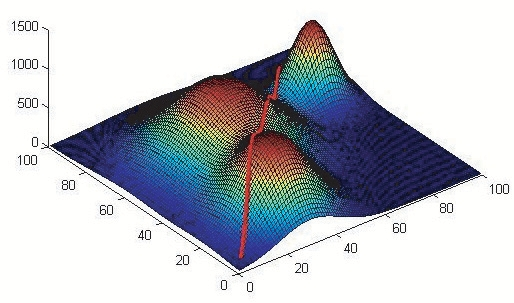
\includegraphics[width=.75\linewidth]{figs/1.jpg}
                  \caption{A 2D world with obstacles depicted as cost functions.
                        Shown in red is a straight line path between two locations.
                        The path has high cost because it passes through/near obstacles.}
                  \label{fig:1}
            \end{figure}

            \begin{figure}[H]
                  \centering
                  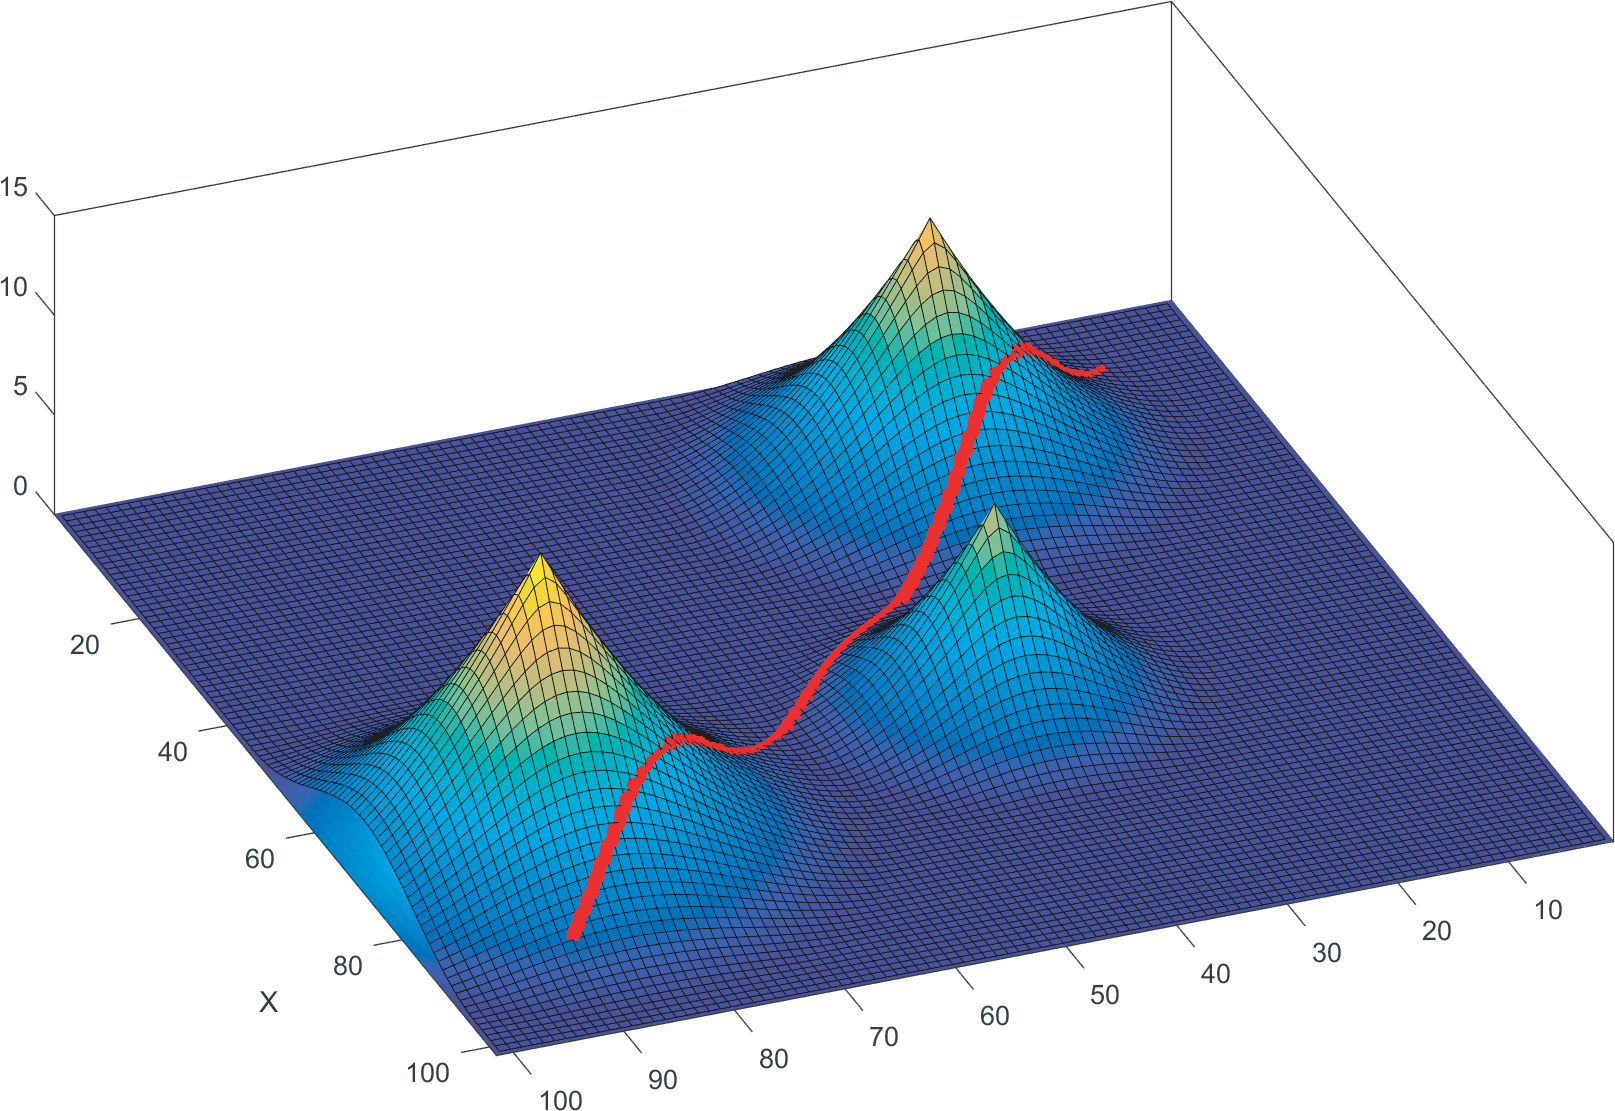
\includegraphics[width=.75\linewidth]{figs/2.png}
                  \caption{Another 2D obstacle world and straight line path with moderately-high cost, corresponding to the code appearing in trajectory\_optimization.$\{$m$\mid$py$\}$.}
                  \label{fig:2}
            \end{figure}

            \begin{enumerate}
                  \item Starting from the straight line path that goes across the obstacle field as in \autoref{fig:2}, perform gradient descent to find a path with locally optimal cost.
                        You should represent the path as a sequence of 2D points, view that sequence as a higher-dimensional point in some finite-dimensional space, and take gradient steps in that space.
                        Rather than optimize along the entire gradient line as we did in lecture, simply scale the negative gradient by 0.1 and take a corresponding step.

                        Remember, this is a path for your robot, so make sure you don't accidentally optimize its start and goal as well; those should remain fixed.

                        Plot the path after one iteration — notice that it is moving away from the obstacles.

                        Pick convergence criteria and plot the path after convergence.
                        What happened to it?
                  \item To avoid the issue from part (a), you need to tell the optimizer that this is a path instead of some independent 2D points.

                        One possibility is to consider an additional cost term, $\min (\frac{1}{2} \|\xi_i - \xi_{i-1}\|^2)$, that tells each 2D point $\xi_i$ to be close to the previous 2D point $\xi_{i-1}$ on the path.
                        This additional term is sometimes called a \textit{smoothness} cost.

                        Augment your negative gradient from part (a) with a new negative gradient, obtained for each $\xi_i$ from the \textit{single} term $\frac{1}{2} \|\xi_i - \xi_i-1\|^2$.

                        (The gradient of this new term with respect to $\xi_i$ is $(\xi_i - \xi_{i-1})$.
                        Include this term for $\xi_i$, but ignore this term when taking a gradient with respect to any other $\xi_j$, including $\xi_{i-1}$.
                        This means we are really specifying a vector field for the optimizer to follow rather than an overall cost function.
                        Another perspective is that each 2D point on the path is optimizing its own cost function, chosen in a convenient way.)

                        Weight the negative obstacle gradient from part (a) with 0.8 and the new negative gradient term with 4, add them together, then again scale that vector by 0.1 and take a corresponding step.
                        (Weights like this are never set in stone; if you wish, you should feel free to experiment with other values.)

                        Plot the path after 100, 200 and 500 iterations.
                        Why doesn't this work?
                  \item Finally, try augmenting the obstacle gradient with a different smoothness cost, telling each 2D point to be close to both its previous and next points on the path:

                        $$
                              \min (\frac{1}{2} \|\xi_i - \xi_{i-1}\|^2 + \frac{1}{2} \|\xi_i+1 - \xi_i\|^2).
                        $$

                        Taking the gradient with respect to $\xi_i$ yields $(\xi_i - \xi_{i-1}) + (\xi_i - \xi_{i+1})$, which is $-\xi_{i-1} + 2\xi_i - \xi_{i+1}$.
                        (We can now view this gradient as derived from an overall cost function or we can again view it as derived for each 2D point from its own cost function.)
                        Perform another optimization using this new smoothness cost to compute gradient
                        updates:
                        \begin{enumerate}
                              \item Use 0.8 to weight the obstacle cost and 4 to weight the smoothness cost.
                                    Then use a step-size scaling of 0.1 as before.
                              \item Again, you should feel free to use different weights if your code works better with those, so long as the weights are not too different from those we suggested.
                        \end{enumerate}
                        Plot the path after 100 and 5000 iterations.
                        Why is this version better?
                  \item What will happen if you were to start the procedure from different initial paths?

                        Will the final answer be the same every time? Why?
                  \item Suppose that the final solution path found by gradient descent, given some initial path and given our original cost function, is not feasible for the robot to execute (it still passes through some high cost regions that you would rather not have the robot pass through)?
                        What simple common-sense strategy can you come up with to try to mitigate this problem?
                        (\textit{No need to write code unless necessary.
                              We expect a very short description of the strategy only.})
            \end{enumerate}

            Please submit code for parts (a), (b), and (c), but none is required for (d) and (e).
            Please provide answers for all parts in your pdf, as usual.
            In particular, replicate any code snippets in your pdf that you think the TAs will need for grading.
\end{enumerate}

\end{document}
